Randomness is \underline{unpredictability}, or \underline{a lack of any discernible pattern}.

Consider the experiment of flipping a coin -- there are two possible outcomes, heads or tails.
This is a \emph{random experiment}, since we cannot predict the outcome.
Moreover a coin flip is not reproducible as an individual event; however it is still possible to understand the relative frequencies of the possible outcomes by repeating this experiment multiple times.
Flipping a fair coin 1000 times, for instance, will give roughly 500 heads and 500 tails.

With a view towards modelling these random experiments, first we discuss random numbers and how to generate them.

\textbf{Question}: Would you characterize the sequence of digits of $\pi$ as \emph{random}?
$$\pi = 3.14159265358979323846\cdots$$
This sequence looks random, in the sense that these digits do not seem to follow any prescribed pattern.
On the other hand, $\pi$ is a fixed number, and any digit of this sequence can be calculated given sufficient resources.
We call such a sequence \emph{pseudorandom}.
This means that the process that outputs digits of $\pi$ in sequence \emph{appears random}, statistically speaking, while being completely deterministic.

In fact, the following process can be used as a [bad] algorithm for generating random numbers from the set $\{0, 1, \ldots, 9\}$:

\begin{algorithm}
\textbf{initialize} $i$ a non-negative integer\;
\textbf{function} rand(): \\
\qquad 	$i \leftarrow i + 1$\;
\qquad	\textbf{return} $i$th digit of $\pi$ \;
\caption{A simple random number generator}
\label{alg:pi}
\end{algorithm}

One nice property of this is algorithm is that as long as we know the initial index $i$, we can repeat exactly the sequence of digits it outputs.
This is called the \emph{seed} of the generator.
This is especially useful for running computer simulations, as sometimes we would like to reproduce results of simulating a random process.
Note that we would not actually use Algorithm~\ref{alg:pi} in a simulation, due to a large part in the computational effort required to compute digits of $\pi$.
Moreover, patterns have been found in its digits\footnote{See \url{http://mathworld.wolfram.com/PiDigits.html}}.
Another simple example is Algorithm~\ref{alg:lin_cong}.


\begin{algorithm}
\textbf{initialize} integers $a$, $m$, $c$ appropriately selected, a seed $x_0$, $i = 0$ \;
\textbf{function} rand(): \\
\qquad $i \leftarrow i + 1$ \;
\qquad $x_{i} = (ax_{i-1} + c)$ \ (mod $m$) \;
\qquad	\textbf{return} $x_i$ \;
\caption{The Linear Congruential Method}
\label{alg:lin_cong}
\end{algorithm}


The $\mod$ here is the \emph{modulo operation} -- it computes the remainder when $(ax_{i-1} + c)$ is divided by $m$.
This means each $x_i$ will be in the set $\{0,1,2,\ldots,m-1\}$.
As in Algorithm~\ref{alg:pi}, Algorithm~\ref{alg:lin_cong} is very easy to replicate, in this case by simply knowing the parameters $a$, $m$, $c$, and the seed $x_0$.

There are certain conditions that these parameters have to satisfy in order to make this algorithm viable.
One desirable property of the produced sequence is a long period, that is, that the algorithm goes through as many values from the set $\{0,1,2,\ldots,m-1\}$ as possible.
For instance, if $c = 0$ and $m$ is prime, the algorithm generates the longest possible period with length $m - 1$ for many values of $a$.\footnote{This holds if $a$ is chosen so that the smallest integer $k$ such that $a^k - 1$ is divisible by $m$ is $k = m - 1$. Such an $a$ is called a \emph{primitive root modulo $m$} -- see \cite{law2015}.}
This algorithm can be modified to output real numbers in $(0,1)$, by dividing the outputs by $m$. 

\begin{myexample} [The Linear Congruential Method]

	Using $a = 6$, $m = 11$, $c = 0$, and $x_0 = 1$, we get the sequence $1, 6, 3, 7, 9, 10, 5, 8, 4, 2,  \ldots$ which goes through all values in $\{1, 2, \ldots, 10\}$ before repeating.

	If we use the same parameters but with $m = 10$ instead, we get $1, 6, 6, 6, \ldots$, reminding us that we need to pay attention to $m$, $a$, and $c$.
\end{myexample}

This example illustrates the operations performed.
Observe that as in Algorithm~\ref{alg:pi}, the output of this algorithm is completely deterministic.
It also becomes more predictable the more numbers you've generated, since you do not repeat $x_i$'s before the period ends (and then after that, the same sequence is produced repeatedly).

In practice however, $m$ is chosen to be very large, and if the other parameters are chosen correctly, the sequence produced will look no different than a random sequence (in the sense that it passes known statistical tests that check for this property).

There are more sophisticated algorithms for random number generation, based on similar ideas to Algorithm~\ref{alg:lin_cong}. 
One popular one is called the \emph{Mersenne Twister}, and which is used by most computational software, including MATLAB, Excel, C++, and others.
For running simulations on a computer, the primary concern in this course is knowing how to use a computer to generate random numbers (although it is helpful understanding how it is done in the background).

\section{Generating Random Numbers in Excel}
In Microsoft Excel, the \texttt{=RAND()} command outputs a random real number\footnote{In computing, real numbers are represented as \emph{floating point numbers} \\ -- see \url{https://en.wikipedia.org/wiki/Floating_point}.} in the interval $[0,1)$.
Whenever the worksheet is re-calculated (by editing a cell, for example), a new real number is returned in this interval.

This function can be in turn used to generate a random real number in any interval $[a,b)$, using the formula \texttt{= a + (b - a)*RAND()}.
Intuitively, this transformation computes the number in the interval $[a,b)$ that is \texttt{RAND()} fraction of the way from $a$ to $b$.

\begin{figure}[htbp]
	\centering
	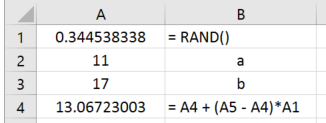
\includegraphics[width=0.45\textwidth]{fig/1_excel_rand.png}
	\caption{Computing random real numbers in Excel}
	\label{fig:excel_rand}
\end{figure}

Note that this process is \emph{not} reproducible; once the worksheet is refreshed, each \texttt{RAND()} call is reset, and the old values cannot be retrieved.
There are two ways of fixing the values generated -- one is to copy and paste these in a separate worksheet; another way is to press F9 after entering the formula instead of Enter.
This makes it so that recalculations are not done when the worksheet is refreshed, and the formula in the cell is overwritten by the computed values.

The type of randomness we discuss in this section is called \emph{uniform}, since numbers from the set under consideration are all \emph{equally likely} to be generated.
We also call this a \emph{uniform distribution} of numbers.

One way of visualizing the random numbers we are generating is by using \emph{histograms}, which are graphs with rectangles or bars representing the frequency of each range of values.
In Figure~\ref{fig:histogram} we show the result of generating 100 real numbers using \texttt{RAND()}, then grouping results into `buckets' $[0,0.1), [0.1,0.2), \ldots, [0.9,1)$. 

\begin{figure}[htbp]
	\centering
	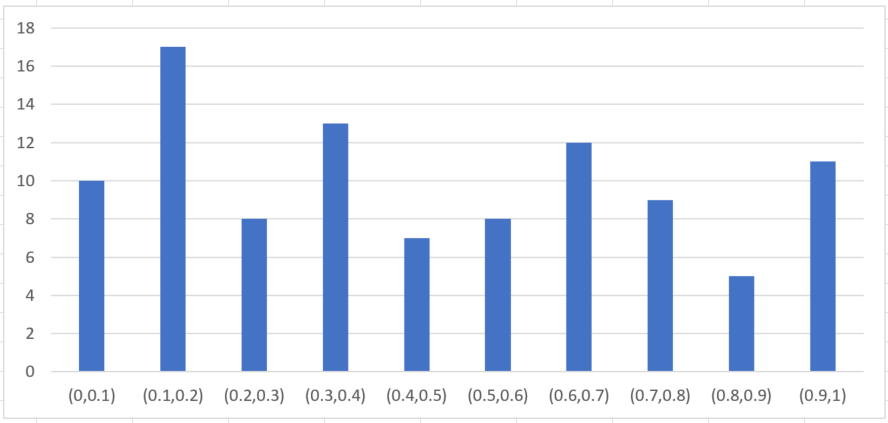
\includegraphics[width=0.6\textwidth]{fig/1_histogram.png}
	\caption{A histogram of one hundred \texttt{RAND()} outputs in Excel \label{fig:histogram}}
\end{figure}

Note that there are 17 numbers in $[0.1,0.2)$ while only 5 in $[0.8,0.9)$.
This is not unusual -- what we would expect the average to be when repeating an experiment multiple times does not necessarily reveal itself in only a few trials.
Observe that the histogram in Figure~\ref{fig:histogram1000}, where we generate a thousand real numbers using \texttt{RAND()}, looks more `evened out.'

\begin{figure}[htbp]
	\centering
	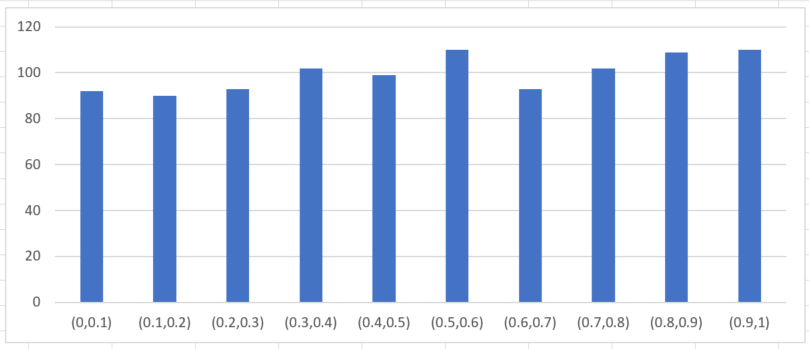
\includegraphics[width=0.6\textwidth]{fig/1_histogram_1000.png}
	\caption{A histogram of one thousand \texttt{RAND()} outputs in Excel \label{fig:histogram1000}}
\end{figure}


In the next section, we will introduce other types of distributions, where some outcomes are more likely than others.
From this point we will use the term \emph{random number} to describe a random real number from $[0,1)$, and the term \emph{random variable} to describe an output that may be generated from any
general probability distribution. 


\begin{center}
	\textbf{EXERCISES}
\end{center}

\begin{enumerate}[label={1.\arabic*},leftmargin=1cm]
	\item \textbf{Explore.} Write a sequence of H's and T's to describe what you think will happen if you flip a coin twenty times. How about fifty? Then actually perform the experiments, and compare the two results. What observations can you make?
	\item An urn contains ten balls - three blue, two green, and five red. \label{exer:1_urn}
		\begin{enumerate}[(a)]
			\item If you pick a ball at random, what are the chances that the ball is blue? red? 
			\item If you pick two balls in succession (without putting back the first ball), what are the chances that the two balls are green?
		\end{enumerate}
	\item What are the chances that you roll a die twice and you never see the number 1? How about three times?
	\item When we take $c = 0$ in Algorithm~\ref{alg:lin_cong}, it is known as the \emph{Multiplicative Congruence Method}, also called the \emph{Lehmer random number generator} after the mathematician D.~H.~Lehmer. A classical choice for its parameters is $m = 2^{31} - 1 = 2147483647$ and $a = 7^5 = 16807$, and this generator has the special name \texttt{MINSTD}. Using Excel, generate the first ten terms of \texttt{MINSTD} when the initial seed is your SFU student ID number. (Divide each term by $m$ so that each output lies in $[0,1)$.) \label{exer:1_Lehmer}
	\item Write a formula in Excel to generate a number uniformly from the following sets:
		\begin{enumerate}[(a)]
			\item The interval $[0, 100)$.
			\item The interval $(-20, -15]$.
			\item The set of integers in the interval $[-20,-15]$.
		\end{enumerate}
	\item Write a formula in Excel that simulates the process of picking a ball at random from the urn in Exercise~\ref{exer:1_urn}
	\item \textbf{Explore.} Replicate the process used in Figure~\ref{fig:histogram} and Figure~\ref{fig:histogram1000} but using different bucket sizes - $0.2$ and $0.05$. That is, generate one hundred, then one thousand random numbers from $[0,1)$, and then aggregate the results using (a) 5 buckets of equal length; (b) 20 buckets of equal length. What do you think the effect of changing the bucket size will be? Compare with the results of your experiment.
	\item Explain the following \texttt{xkcd} comic:
		\begin{figure}[htbp]
			\centering
			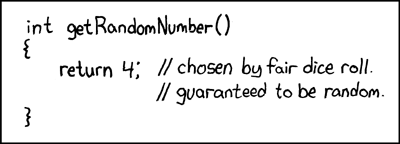
\includegraphics[width=0.5\textwidth]{fig/1_xkcd_random_number.png}
			\captionsetup{labelformat=empty}
			\label{fig:xkcd_random}
			\caption{Source: \texttt{https://xkcd.com/221/}}
		\end{figure}
\end{enumerate}


